\begin{center}
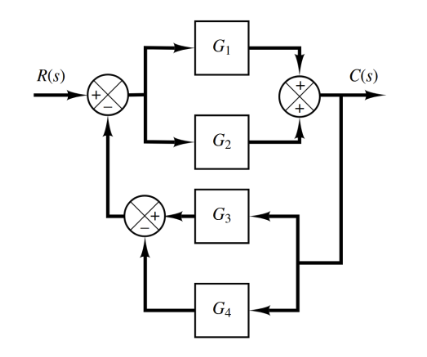
\includegraphics[width=0.5\linewidth]{figs/6.png}
\end{center}
بر اساس دیاگرام، سیگنال \(E(s)\) پس از جمع‌کنندهٔ اول (ورودی \(R(s)\) مثبت و فیدبک منفی) به دو شاخهٔ موازی \(G_1\) و \(G_2\) می‌رود؛ خروجی‌ها با هم جمع می‌شوند، پس:
\[
C(s)=G_1 E(s)+G_2 E(s)=(G_1+G_2)E(s)
\]

سیگنال \(C(s)\) به مسیر فیدبک نیز می‌رود؛ خروجی \(G_3\) با علامت مثبت و خروجی \(G_4\) با علامت منفی در جمع‌کنندهٔ فیدبک ترکیب می‌شوند:
\[
B(s)=G_3 C(s)-G_4 C(s)=(G_3-G_4)C(s)
\]

برای جمع‌کنندهٔ اول داریم:
\[
E(s)=R(s)-B(s)=R(s)-(G_3-G_4)C(s)
\]

با جایگذاری در رابطهٔ \(C(s)=(G_1+G_2)E(s)\):
\[
C(s)=(G_1+G_2)\bigl[R(s)-(G_3-G_4)C(s)\bigr]
\]
\[
C(s)=(G_1+G_2)R(s)-(G_1+G_2)(G_3-G_4)C(s)
\]

انتقال جملهٔ حاوی \(C(s)\) به یک طرف:
\[
C(s)+(G_1+G_2)(G_3-G_4)C(s)=(G_1+G_2)R(s)
\]
\[
C(s)\Bigl[1+(G_1+G_2)(G_3-G_4)\Bigr]=(G_1+G_2)R(s)
\]

پس معادل حلقهٔ استاندارد برابر است با:
\[
\boxed{
\frac{C(s)}{R(s)}=
\frac{G_1+G_2}
{1+(G_1+G_2)(G_3-G_4)}
}
\]
